\documentclass{math}

\usepackage{tikz}

\title{University Physics 1A}
\author{Alvin Lin}
\date{November 16th, 2017}

\begin{document}

\maketitle

\section*{Torque Concepts}
If an object is in static equilibrium, its acceleration is 0. The net force on
the object is 0 and the object is not rotating around any point. When
calculating torque, it is important what point you choose as the pivot point
or reference point because the torque calculated is different for each reference
point.

\subsubsection*{Example}
Suppose we have a rod of mass \( m \) and length \(L \) a hinge and suspended
by a string. Choosing the point \( \frac{L}{4} \) as our pivot point in the
problem gives the following equations.
\begin{center}
  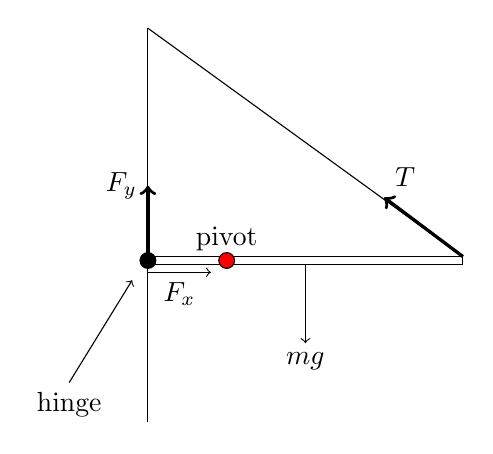
\begin{tikzpicture}
    \draw (0,0) -- (0,5);
    \draw (0,2) -- (4,2) -- (4,2.1) -- (0,2.1) -- cycle;
    \draw[fill=black] (0,2.05) circle (0.1cm);
    \draw (4,2.1) -- (0,5);
    \draw[very thick,->] (4,2.1) -- (3,2.85) node[above right] {\( T \)};
    \draw[->] (2,2) -- (2,1) node[below] {\( mg \)};
    \draw[->] (0,1.9) -- (0.8,1.9) node[below,pos=0.5] {\( F_x \)};
    \draw[very thick, ->] (0,2) -- (0,3) node[left] {\( F_y \)};
    \draw[->] (-1,0.5) -- (-0.2,1.8) node[pos=0,below]{hinge};
    \draw[fill=red] (1,2.05) circle (0.1cm) node[above] {pivot};
  \end{tikzpicture}
\end{center}
\begin{align*}
  F_{net~y} &= F_y-mg+T\sin\theta = 0 \\
  F_{net~x} &= F_x-T\sin\theta = 0 \\
  \tau_{net} &= -F_y\frac{L}{4}-mg\frac{L}{4}+T\sin\theta\frac{3L}{4} = 0 \\
  0 &= -(mg-T\sin\theta)\frac{L}{4}-\frac{mgL}{4}+\frac{3TL}{4}\sin\theta \\
  &= -mg\frac{L}{4}+\frac{TL}{4}\sin\theta-\frac{mgL}{4}+
    \frac{3TL}{4}\sin\theta \\
  mg\frac{L}{4}+mg\frac{L}{4} &= \frac{TL}{4}\sin\theta(4) \\
  \frac{1}{2}mgL &= TL\sin\theta \\
  T &= \frac{mg}{2\sin\theta}
\end{align*}

It is much easier to choose the pivot point at the location of an unknown force
to simplify the algebra. Suppose we choose the hinge as our pivot point.
\begin{center}
  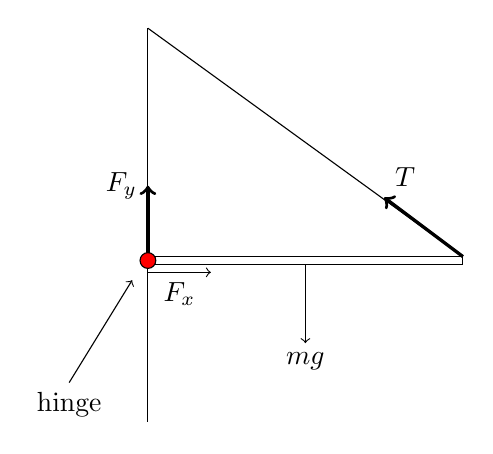
\begin{tikzpicture}
    \draw (0,0) -- (0,5);
    \draw (0,2) -- (4,2) -- (4,2.1) -- (0,2.1) -- cycle;
    \draw (4,2.1) -- (0,5);
    \draw[very thick,->] (4,2.1) -- (3,2.85) node[above right] {\( T \)};
    \draw[->] (2,2) -- (2,1) node[below] {\( mg \)};
    \draw[->] (0,1.9) -- (0.8,1.9) node[below,pos=0.5] {\( F_x \)};
    \draw[very thick, ->] (0,2) -- (0,3) node[left] {\( F_y \)};
    \draw[->] (-1,0.5) -- (-0.2,1.8) node[pos=0,below]{hinge};
    \draw[fill=red] (0,2.05) circle (0.1cm);
  \end{tikzpicture}
\end{center}
The force equations remain the same no matter what, but the net torque becomes:
\begin{align*}
  \tau_{net} &= 0 = 0-mg\frac{L}{2}+T\sin\theta \\
  T &= \frac{mg}{2\sin\theta}
\end{align*}

Suppose the weight supported by the string is 1.5 times the tension calculated.
How far can a person with weight \( \frac{3m}{5} \) walk along the rod before
the string snaps?
\begin{center}
  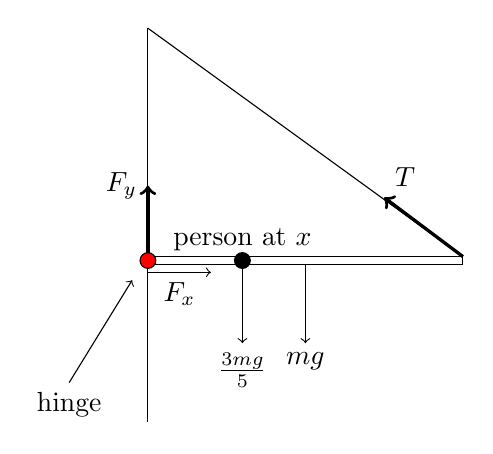
\begin{tikzpicture}
    \draw (0,0) -- (0,5);
    \draw (0,2) -- (4,2) -- (4,2.1) -- (0,2.1) -- cycle;
    \draw (4,2.1) -- (0,5);
    \draw[very thick,->] (4,2.1) -- (3,2.85) node[above right] {\( T \)};
    \draw[->] (2,2) -- (2,1) node[below] {\( mg \)};
    \draw[->] (0,1.9) -- (0.8,1.9) node[below,pos=0.5] {\( F_x \)};
    \draw[very thick, ->] (0,2) -- (0,3) node[left] {\( F_y \)};
    \draw[->] (-1,0.5) -- (-0.2,1.8) node[pos=0,below]{hinge};
    \draw[fill=red] (0,2.05) circle (0.1cm);
    \draw[fill=black] (1.2,2.05) circle (0.1cm) node[above] {person at \( x \)};
    \draw[->] (1.2,2.05) -- (1.2,1) node[below] {\( \frac{3mg}{5} \)};
  \end{tikzpicture}
\end{center}
\begin{align*}
  T_{max} &= \left(\frac{3}{2}\right)\left(\frac{mg}{2\sin\theta}\right) \\
  F_{net~y} &= F_y-mg+T\sin\theta-\frac{3mg}{5} \\
  F_{net~x} &= F_x-T\cos\theta = 0 \\
  \tau_{net} &= 0-mg\frac{L}{2}+T_{max}sin(\theta) L-\frac{3}{5}mgx = 0 \\
  &= -\frac{mgL}{2}+\frac{3}{2}\frac{mg}{2\sin\theta}\sin\theta L-
    \frac{3}{5}mgx \\
  \frac{mgL}{2}-\frac{3}{4}mgL &= -\frac{3}{5}mgx \\
  x &= -\frac{5}{3}\left(\frac{L}{2}-\frac{3}{4}L\right) \\
  &= \frac{5}{12}L
\end{align*}
The person can only walk \( \frac{5}{12} \) of the way along the rod.

\begin{center}
  You can find all my notes at \url{http://omgimanerd.tech/notes}. If you have
  any questions, comments, or concerns, please contact me at
  alvin@omgimanerd.tech
\end{center}

\end{document}
